\chapter{Giới thiệu}

\section{Giới thiệu đề tài}


Ngày nay, bùng nổ dân số và xu hướng đô đô thị hóa nhanh, dân số tập trung đông tại các thành phố lớn
đòi hỏi yêu cầu phát triển cơ sở hạ tầng giao thông để đảm bảo đô thị được vận hành hiệu quả.
Khi hệ thống giao thông ngày càng mở rộng và phát triển, thì các nhà quy hoạch và quản lý đô thị càng quan tâm 
tới bài toán giám sát một mạng lưới giao thông phức tạp của thành phố, đảm bảo cho hệ thống phải an toàn và thông suốt.
Các tình huống thường gặp trên đường bao gồm ùn tắc giao thông, vượt đèn đỏ, lái xe quá tốc độ dẫn đến tai nạn và
không đội mũ bảo hiểm với xe máy và thậm chí là truy vết tội phạm đang tham gia giao thông.
Do đó, giám sát giao thông là một bài toán cơ bản, quan trọng và không thể thiếu với các đô thị lớn nhằm đảm bảo giao thông được vận hành hiệu quả.

\begin{figure}[H]
    \centering
    \includegraphics[width=0.75\textwidth]{images/CCTV.jpg}
    \caption[Camera giám sát trên đường Vành đai 3 Hà Nội]{Camera giám sát trên đường Vành đai 3, Hà Nội. Hiện nay, thành phố Hà Nội triển khai các camera giám sát trên diện rộng hướng đến mục tiêu giám sát giao thông tự động toàn thành phố.}
    \label{fig:traffic}
\end{figure}

Trong một thời gian rất dài trước đây, tại những thành phố lớn, việc giám sát giao thông chủ yếu dựa vào
lực lượng chức năng túc trực trên các tuyến đường và nút giao thông trọng điểm để quan sát, phát hiện và xử lý vi phạm.
Cách tiệp cận truyền thống này phụ thuộc lớn vào số lượng nhân lực và khó đảm bảo khả năng theo dõi trên toàn bộ đô thị.
Tại Việt Nam, từ lâu chính quyền đã cho lắp đặt camera an ninh ở một vài vị trí để theo dõi tình hình giao thông.
Tuy nhiên, việc lắp đặt các camera giám sát một cách có có hệ thống cho việc giám sát tự động chỉ mới được triển khai trong những năm gần đây,
hướng đến mục tiêu giám sát tự động và ra quyết định theo thời gian thực.
Tuy vậy, triển khai giám sát bằng camera trên diện rộng đặt ra nhiều vấn đề và thách thức, trong đó có vấn đề về xử lý
lượng dữ liệu lớn và liên tục trong thời gian thực, có thể gây tắc nghẽn cho hệ thống và làm sai lệch kết quả giám sát.

\begin{figure}[H]
    \centering
    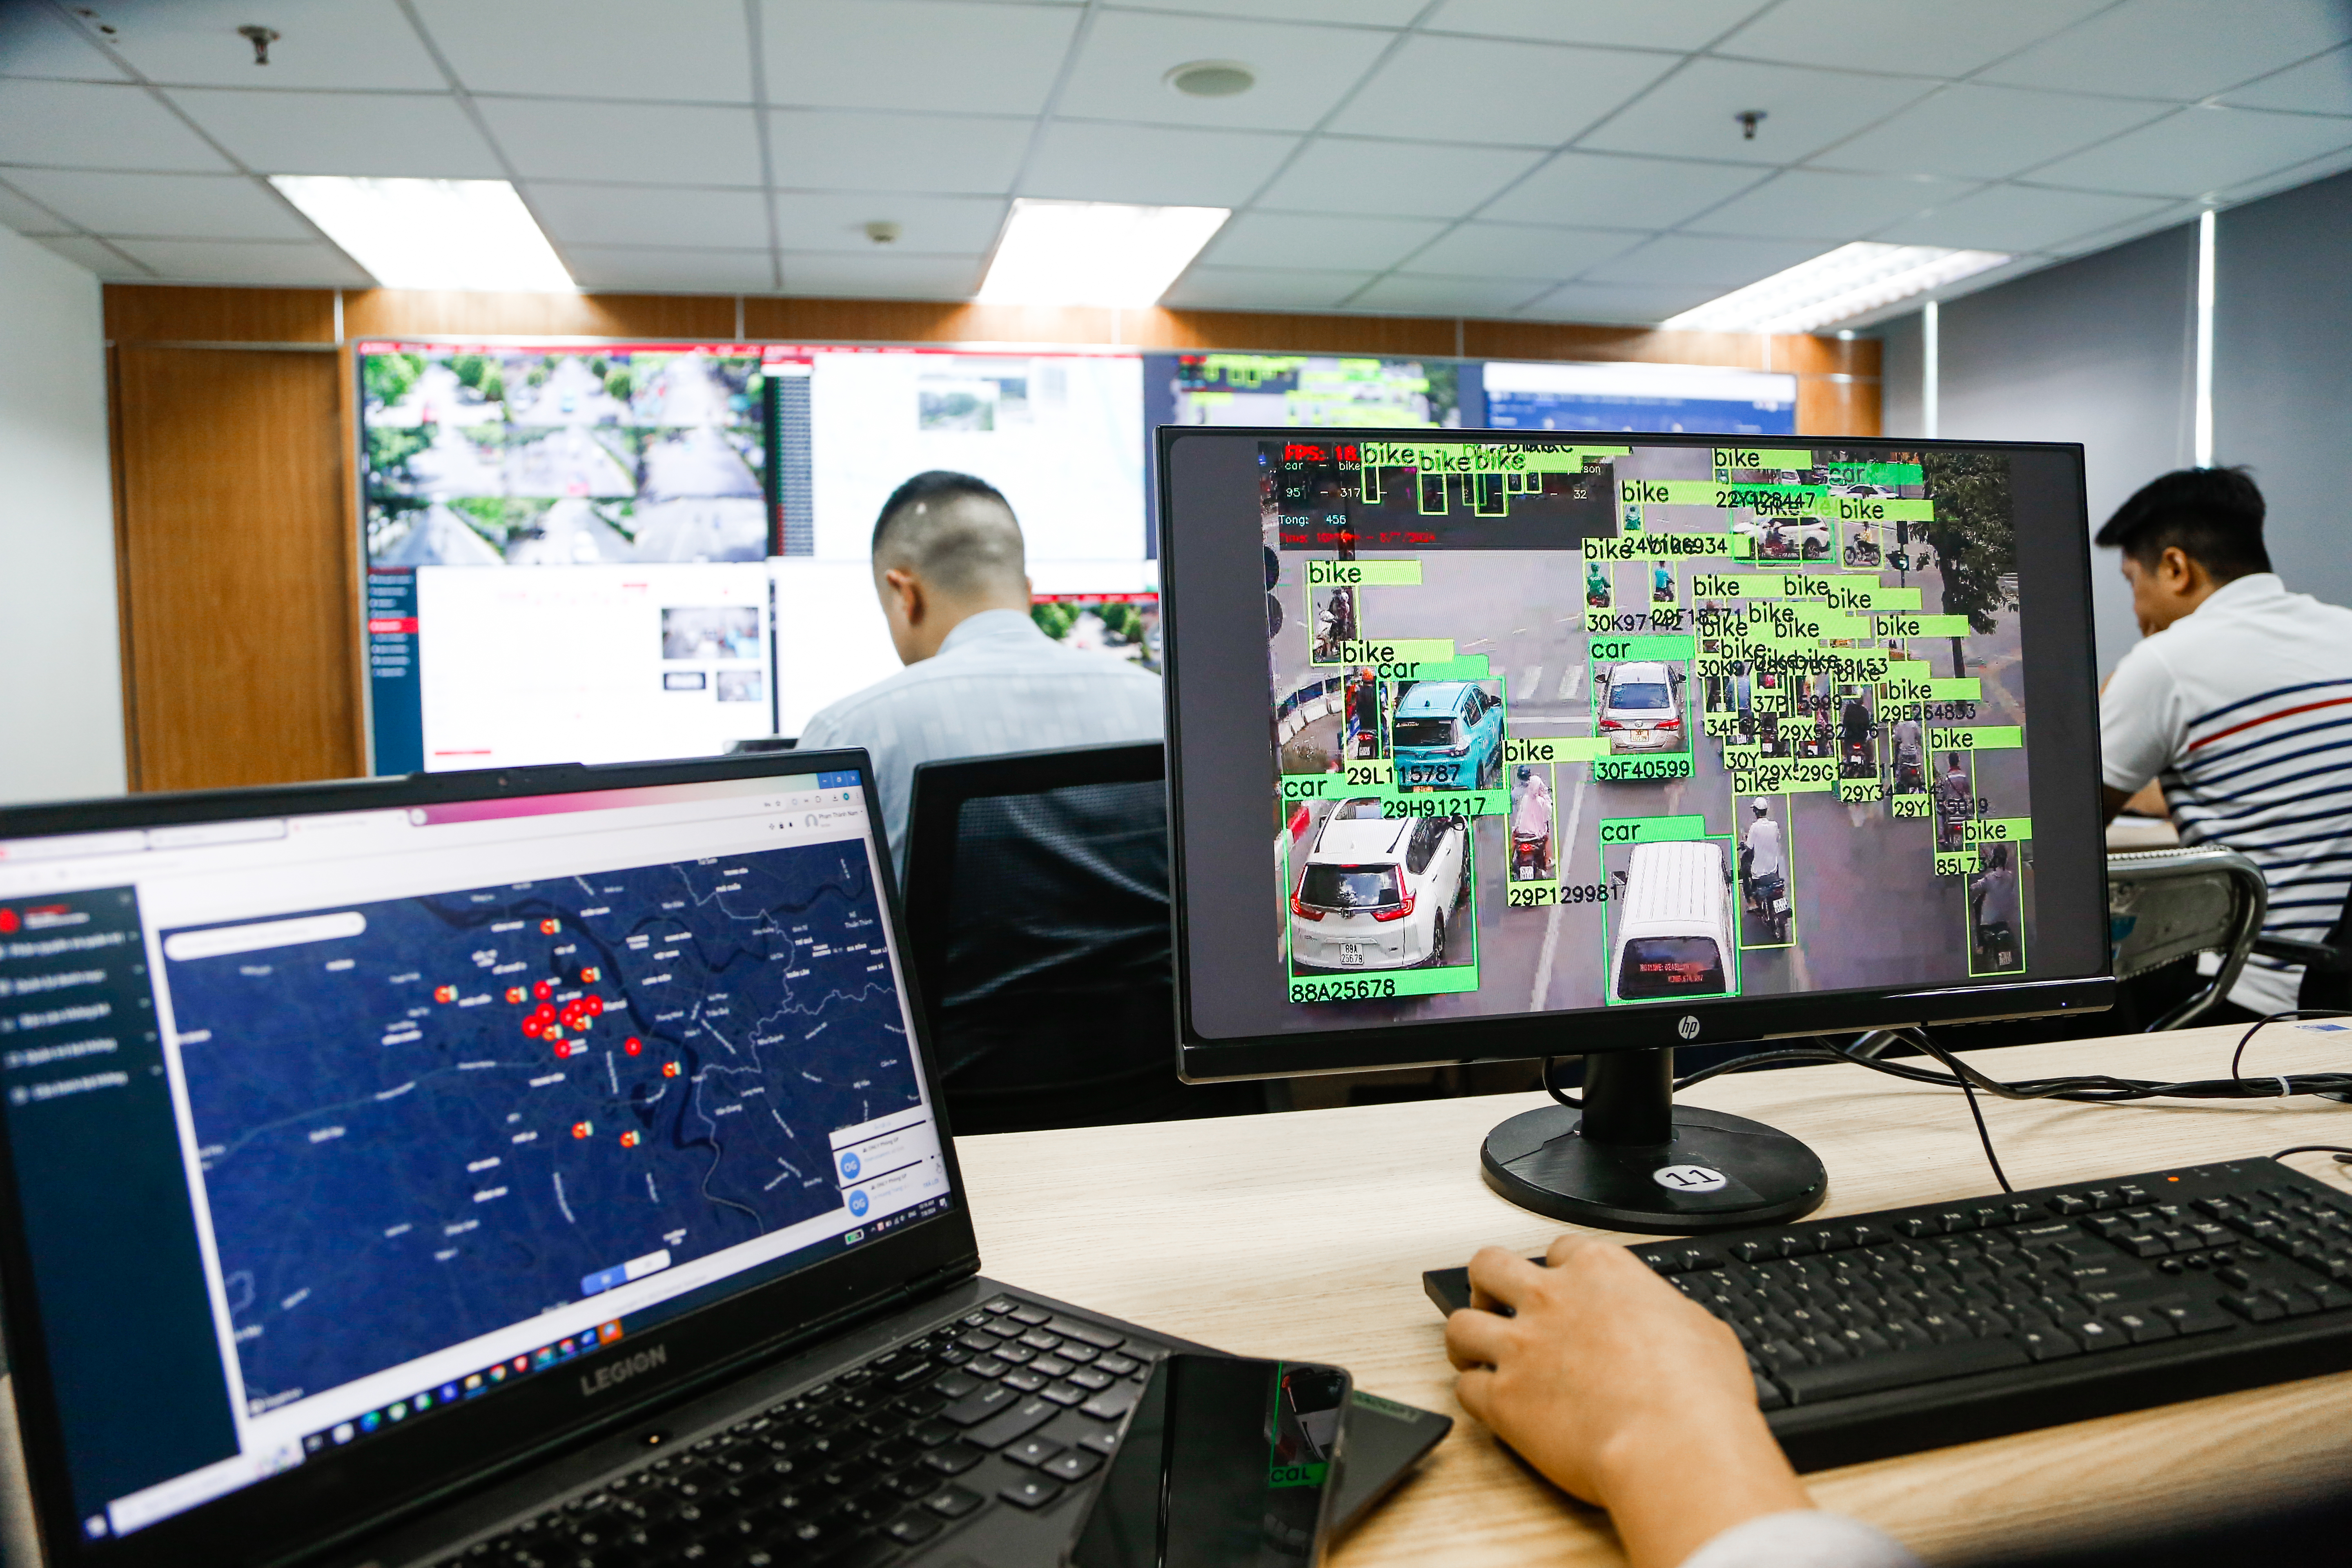
\includegraphics[width=0.85\textwidth]{images/TrungTamDieuHanhHaNoi.png}
    \caption[Trung tâm Điều hành giao thông thông minh Hà Nội]{Bên trong Trung tâm Điều hành giao thông thông minh tại Thành phố Hà Nội, một cán bộ đang theo dõi các phương tiện trên màn hình máy tính.}
    \label{fig:MonitorCentral}
\end{figure}

Trong lĩnh vực Học sâu và Thị giác máy tính, mô hình YOLO là một trong những mô hình tiên tiến cho bài toán nhận diện cũng như theo dõi vật thể trong thời gian thực,
có thể được áp dung trong các bài toán giám sát giao thông như nhận diện biển số xe, phát hiện vượt đèn đò hoặc chạy vượt quá tốc độ, phát hiện không đội mũ khi đi xe máy,
cũng như đếm lưu lượng phương tiện để cảnh báo ùn tắc.
Với một lượng dữ liệu lớn cần xử lý trong thời gian thực, ta có các công nghệ dữ liệu lớn như Apache Kafka kết hợp với Apache Flink
cung cấp nền tảng xử lý thời gian thực với độ trễ thấp, khả năng mở rộng quy mô và khả năng chịu lỗi cao. Khối lượng dữ liệu lớn đó có thể được lưu trữ và truy vấn hiệu quả
thông qua MongoDB, một cơ sở dữ liệu NoSQL được sử dụng nhờ tính linh hoạt với dữ liệu phi cấu trúc.

\newpage
\section{Phát biểu bài toán}

Bài toán ``Giám sát giao thông thời gian thực sử dụng công nghệ dữ liệu lớn và học sâu'' được phát biểu như sau:

\begin{enumerate}
    \item \textit{Đầu vào}: Là một dữ liệu video/hình ảnh được thu thập từ camera giám sát giao thông trên các tuyến đường hoặc tại nút giao, có chứa các phương tiện đang di chuyển trên đường.
    Các video/hình ảnh có độ phân giải và điều kiện quay chụp khác nhau, và đều được truyền phát liên tục từng khung hình trong thời gian thực.
    \item \textit{Đầu ra}: Nhật ký thông tin các phương tiện di chuyển qua đoạn đường, bao gồm biển số xe, ngày giờ di chuyển, các lỗi vi phạm; Báo cáo tình trạng giao thông trên mỗi tuyến đường/nút giao mà camera truyền phát đến.
    \item \textit{Yêu cầu}: Sử dụng các mô hình học sâu để thực hiện các bài toán theo dõi và nhận diện vật thể một cách chính xác; 
    Tích hợp các công nghệ dữ liệu lớn để xử lý song song, phân tán các khung hình nhằm xử lý dữ liệu theo thời gian thực;
    Lưu trữ các thông tin đã qua nhận diện hoặc xử lý vào cơ sở dữ liệu để sẵn dùng cho các tác vụ khác.
\end{enumerate}

Bài toán này có thể được phát biểu theo nhiều cách khác nhau, nhưng chúng tôi sẽ lấy phát biểu trên làm cơ sở để tiến hành quá trình tìm hiểu và nghiên cứu các giải pháp liên quan.
Phạm vi và mục tiêu nghiên cứu sẽ được trình bày cụ thể hơn ở phần sau. 



\section{Các nghiên cứu liên quan}

Trong nhiều năm qua, giám sát giao thông đã trở thành một trong những bài toán nghiên cứu và ứng dụng quan trọng góp phần hỗ trợ và thúc đẩy phát triển các thành phố thông minh, hiện đại.
Trong số đó, có nhiều công trình nghiên cứu không chỉ các thuật toán phát hiện mà còn khai thác các nền tảng tính toán phân tán và công nghệ dữ liệu lớn
để xây dựng hệ thống giám sát thời gian thực.
Chúng tôi đã thực hiện thu thập và phân tích một cách có hệ thống nhiều công trình nghiên cứu liên quan, tập trung vào bài toán chính giám sát giao thông và các bài toán cấu thành bao gồm
nhận dạng biển số xe, phát hiện vi phạm giao thông, ước lượng mật độ giao thông và xây dựng hệ thống xử lý dữ liệu lớn trong thời gian thực.

Bài toán xử lý dữ liệu giao thông thời gian thực sử dụng Apache Kafka và Flink đã được khám phá trong công trình của Gnana Deepthi và cộng sự (2023) \cite{Deepthi2024}. 
Các tác giả đề xuất kiến trúc FRTSPS (Flexible Real-Time Traffic Stream Processing System), cho phép xử lý đồng thời dữ liệu theo lô (batch processing) và dữ liệu theo luồng (stream processing) từ các camera giao thông. 
Kiến trúc này giúp giảm độ trễ và tăng khả năng mở rộng, với Kafka đóng vai trò là bộ đệm dữ liệu đầu vào để quản lý luồng dữ liệu liên tục từ nguồn như camera. 
Sau đó, Flink thực hiện các phép biến đổi như map, filter hay reduce để phân tích các chỉ số như lưu lượng xe, tốc độ trung bình và vị trí phương tiện tại các khoảng thời gian cụ thể. 
Thực nghiệm cho thấy FRTSPS có độ trễ thấp hơn so với các nền tảng như Apache Spark hay Storm. 
Công trình này cho thấy khả năng của Flink trong xử lý dữ liệu giao thông, gợi ý rằng nó có thể áp dụng để phát triển hệ thống giám sát giao thông thông minh tại các đô thị lớn.

\section{Mục tiêu và phạm vi dự án}

\subsection{Mục tiêu dự án}

Mục tiêu tổng quát của đề tài ``Giám sát giao thông thời gian thực sử dụng công nghệ dữ liệu lớn và học sâu'' là xây dựng một hệ thống có khả năng giám sát giao thông tự động
thông qua hệ thống các thiết bị biên. Hệ thống phải có khả năng hoạt động với lượng dữ liệu lớn, nhiều nguồn, hoạt động liên tục trong thời gian thực với độ trễ chấp nhận được,
trong đó được áp dụng hay tích hợp các công nghệ về xử lý dữ liệu lớn và học sâu.
Từ đó cung cấp một giải pháp cơ bản hỗ trợ các cơ quan chức năng trong việc giám sát giao thông tự động.


Mục tiêu cụ thể của dự án này là xây dựng một hệ thống giám sát giao thông tự động dựa trên một hệ thống nhiều camera khác nhau, có khả năng theo dõi các phương tiện,
phát hiện các vi phạm (nếu có), phân tích tình trạng giao thông với dữ liệu được gửi liên tục từ hệ thống camera đó trong thời gian thực. Trong đó:

\begin{itemize}
    \item \textit{Xử lý dữ liệu luồng theo thời gian thực}: Tích hợp Apache Kafka để thu thập và truyền phát dữ liệu liên tục theo thời gian thực, với khả năng truyền phát thông tin liên tục từ nhiều nguồn khác nhau cùng lúc;
    Sử dụng Apache Flink để xử lý dữ liệu luồng thời gian thực với hiệu suất cao và khả năng mở rộng dễ dàng khi lượng dữ liệu tăng cao.
    \item \textit{Huấn luyện mô hình học sâu}: Huấn luyện, triển khai mô hình YOLO cùng các thuật toán tracking cho việc theo dõi chuyển động của các phương tiện, phân tích tình trạng giao thông với tốc độ xử lý nhanh; 
    Huấn luyện, triển khai mô hình CNN sâu và các thuật toán khác để nhận diện biển kí tự biển số xe và nhận diện các lỗi vi phạm với độ chính xác cao.
    
    \item \textit{Lưu trữ dữ liệu}: Lưu trữ các kết quả sau khi đã nhận diện, phân tích vào MongoDB, giúp quản lý và truy xuất thông tin giao thông về sau dễ dàng và hiệu quả.
    
\end{itemize}



\subsection{Phạm vi thực hiện}

Do luôn tồn tại sự cản trở tự nhiên về mặt địa lý, giới hạn về dữ liệu và tài nguyên tính toán, nên mục này đặt ra một số phạm vi hoặc giới hạn hiện có trong dự án này.

Về dữ liệu đầu vào:

\begin{itemize}
    \item Video đường phố hoặc ngã tư, được ghi hình theo thời gian thực bởi camera, tập trung chủ yếu vào giao thông trong đô thị tại Việt Nam.
    \item  
\end{itemize}

Công nghệ và công cụ sử dụng:
\begin{itemize}
    \item Ngôn ngữ chính: Python
    \item Xử lý ảnh và học sâu: OpenCV, Ultralytics, PyTorch.
    \item Xử lý dữ liệu: Apache Kafka, Apache Flink, MongoDB.
    \item Môi trường triển khai: Docker, WSL Ubuntu.
\end{itemize}

Giới hạn nghiên cứu:
\begin{itemize}
    \item Nghiên cứu tập trung vào bài toán xử lý luồng dữ liệu trong thời gian thực, chưa tập trung vào xây dựng mô hình học sâu tối ưu cho bài toán.
    \item Nghiên cứu dừng lại ở một hệ thống thực hiện xử lý luồng dữ liệu từ lúc nó được sinh ra ở camera cho tới khi đến được trình giám sát và lưu vào cơ sở dữ liệu, chưa tích hợp vào một hệ thống quản lý giao thông lớn hơn.
    \item Nghiên cứu chưa mở rộng sang các thiết bị biên khác, chưa mở rộng đối với giao thông nước ngoài.
\end{itemize}

Với phạm vi thực hiện này, đề tài hướng đấy xây dựng một hệ thống giám sát giao thông có thể xử lý một luồng dữ liệu lớn trong thời gian, với độ tin cậy và khả năng chịu lỗi cao,
đồng thời áp dụng các mô hình học sâu cho từng bài toán, đảm bảo tính ứng dụng cao trong thực tế.

\section{Phương pháp thực hiện}

\subsection{Phương pháp nghiên cứu lý thuyết}

Tìm hiểu và tổng hợp các nghiên cứu liên quan đến bài toán giám sát giao thông tự động trong thành phố, đặc biệt là các phương pháp sử dụng các công nghệ dữ liệu lớn.

Tìm hiểu các thuật toán, mô hình học sâu để giải quyết các bài toán con của giám sát giao thông.

Nghiên cứu các công nghệ xử lý dữ liệu lớn như Apache Kafka, Apache Flink, MongoDB để đảm bảo hệ thống có khả năng hoạt động với dữ liệu luồng theo thời gian thực.

\subsection{Phương pháp triển khai}

\subsection{Phương pháp thực nghiệm và đánh giá}



